\documentclass{ximera}

\newcommand{\RR}{\mathbb R}
\renewcommand{\d}{\,d}
\newcommand{\dd}[2][]{\frac{d #1}{d #2}}
\renewcommand{\l}{\ell}
\newcommand{\ddx}{\frac{d}{dx}}
\newcommand{\dfn}{\textbf}
\newcommand{\eval}[1]{\bigg[ #1 \bigg]}


\author{Jim Talamo}

\outcome{Answer conceptual questions about arc length.}

\begin{document}
\begin{exercise}

Select all of the following statements that are true.

\begin{selectAll}
\choice[correct]{If $\vec{p}(t)$ uses arc length as a parameter and $\uvec{t}(t)$ denotes the \emph{unit} tangent vector, then $\uvec{t}(t) = \vec{p}'(t)$.}
\choice[correct]{If $\vecl(t) = \vec{v}t+\vec{P}_0$ is an arc length parameterization of a line, then $\vec{v}$ \emph{must} be a unit vector.}
\choice{If the curve $C$ is traced out by $\vec{r}(t) = \vector{t^2,\frac{1}{2}t}, -\infty < t < \infty$, then the curve is parameterized by arc length since \[ |\vec{r}'(t)| = \sqrt{4t^2+\frac{1}{4}} = 1 \textrm{  when } t = \frac{\sqrt{3}}{4}. \]}
\choice{If the curve $C$ is parameterized by $\vec{p}(t)$, and it is known that $\vec{p}(0) = \vector{0,0}$ and $\vec{p}(3) = \vector{2,4}$, it is possible that $\vec{p}(t)$ is an arc length parameterization.}
\choice[correct]{If the curve $C$ is parameterized by $\vec{p}(t)$, and it is known that $\vec{p}(0) = \vector{0,0}$ and $\vec{p}(8) = \vector{2,4}$, it is possible that $\vec{p}(t)$ is an arc length parameterization.}
\end{selectAll}
(Use the hint to see the logic behind each choice)

\begin{hint}


\begin{question}
For the statement

\begin{quote}
True or False: If $\vec{p}(t)$ uses arc length as a parameter and $\uvec{t}(t)$ denotes the \emph{unit} tangent vector, then $\uvec{t}(t) = \vec{p}'(t)$
\end{quote}
do you want to see an explanation?

\begin{multipleChoice}
\choice[correct]{Yes.}
\choice{No}
\end{multipleChoice}

\begin{feedback}[correct]
In general, the unit tangent vector is given by

\[
\uvec{t}(t) = \frac{\vec{p}'(t)}{\left|\vec{p}'(t)\right|}.
\]
Since $\vec{p}(t)$ uses arc length as a parameter, we have that $\left|\vec{p}'(t)\right| = \answer{1}$.

\end{feedback}
\end{question}
%%%%%%%%%%%%%%%%%%%%%%%%%%%%%%%%%%%%%%%%%%%%%%%%%%%%


\begin{question}
For the statement

\begin{quote}
True or False: If $\vecl(t) = \vec{v}t+\vec{P}_0$ is an arc length parameterization of a line, then $\vec{v}$ \emph{must} be a unit vector.
\end{quote}
do you want to see an explanation?

\begin{multipleChoice}
\choice[correct]{Yes.}
\choice{No}
\end{multipleChoice}

\begin{feedback}[correct]
If $\vecl(t)$ is an arc length parameterization, $\left|\vecl'(t)\right| = \answer{1}$.  Since the $\vec{v}$ and $\vec{P}_0$ are constant vectors, 

\[
\vecl'(t) = \vec{v}.
\]

Hence, $\left|\vecl'(t)\right| = \left|\vec{v}\right|$ for all $t$.

\end{feedback}
\end{question}
%%%%%%%%%%%%%%%%%%%%%%%%%%%%%%%%%%%%%%%%%%%%%%%%%%%%


\begin{question}
For the statement

\begin{quote}
True or False: If the curve $C$ is traced out by $\vec{r}(t) = \vector{t^2,\frac{1}{2}t}, -\infty < t < \infty$, then the curve is parameterized by arc length since 

\[ |\vec{r}'(t)| = \sqrt{4t^2+\frac{1}{4}} = 1 \textrm{  when } t = \frac{\sqrt{3}}{4}. \]
\end{quote}
do you want to see an explanation?

\begin{multipleChoice}
\choice[correct]{Yes.}
\choice{No}
\end{multipleChoice}

\begin{feedback}[correct]
The calculation is correct; since $\vec{r}(t) = \vector{t^2,\frac{1}{2}t}$, we have

\[
\vec{r}'(t) = \vector{2t,\frac{1}{2}}.
\]
Thus, $|\vec{r}'(t)| = \sqrt{(2t)^2+\left(\frac{1}{2}\right)^2} = \sqrt{4t^2+\frac{1}{4}}$.

However, the curve is parameterized by arc length if and only if $|\vec{r}'(t)| =1$ for \emph{all} $t$, not just a specific $t$-value.
\end{feedback}
\end{question}
%%%%%%%%%%%%%%%%%%%%%%%%%%%%%%%%%%%%%%%%%%%%%%%%%%%%


\begin{question}
For the statement

\begin{quote}
True or False: If the curve $C$ is parameterized by $\vec{p}(t)$, and it is known that $\vec{p}(0) = \vector{0,0}$ and $\vec{p}(3) = \vector{2,4}$, it is possible that $\vec{p}(t)$ is an arc length parameterization.
\end{quote}
do you want to see an explanation?

\begin{multipleChoice}
\choice[correct]{Yes.}
\choice{No}
\end{multipleChoice}

\begin{feedback}[correct]
If the curve uses arc length as a parameter, $\vec{p}(3)$ should give us the position $(x,y)$ after we have travelled $3$ units along the curve.  The question is, can we travel from the points associated to $\vec{p}(0)$ and $\vec{p}(3)$ by going exactly $3$ units?

Note, the shortest distance between the points associated to $\vec{p}(0)$ and $\vec{p}(3)$ is the length of the line segment between them, and this line segment has length

\[
\sqrt{(2-0)^2+(4-0)^2} = \sqrt{20} >3.
\]

\end{feedback}
\end{question}
%%%%%%%%%%%%%%%%%%%%%%%%%%%%%%%%%%%%%%%%%%%%%%%%%%%%



\begin{question}
For the statement

\begin{quote}
True or False: If the curve $C$ is parameterized by $\vec{p}(t)$, and it is known that $\vec{p}(0) = \vector{0,0}$ and $\vec{p}(8) = \vector{2,4}$, it is possible that $\vec{p}(t)$ is an arc length parameterization.
\end{quote}
do you want to see an explanation?

\begin{multipleChoice}
\choice[correct]{Yes.}
\choice{No}
\end{multipleChoice}

\begin{feedback}[correct]
If the curve uses arc length as a parameter, $\vec{p}(8)$ should give us the position $(x,y)$ after we have travelled $8$ units along the curve.  The question is, can we travel from the points associated to $\vec{p}(0)$ and $\vec{p}(8)$ by going exactly $8$ units?

Note, the shortest distance between the points associated to $\vec{p}(0)$ and $\vec{p}(8)$ is the length of the line segment between them, and this line segment has length

\[
\sqrt{(2-0)^2+(4-0)^2} = \sqrt{20} <8.
\]

It thus should be possible.  

In fact, an explicit example is obtained geometrically by tracing along the segment below at a rate of one unit of distance per unit of time, so we trace out a border of each block each unit of time.

\begin{image}
    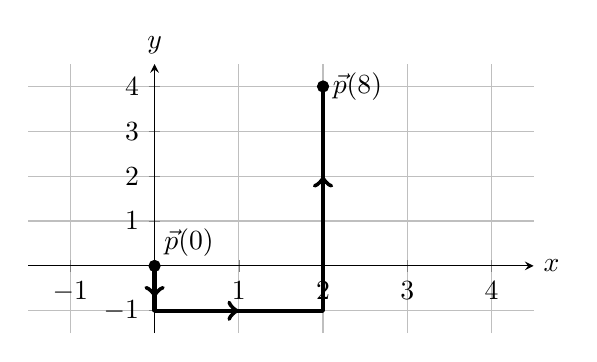
\begin{tikzpicture}
      \begin{axis}%
        [
	  xmin=-1.5,xmax=4.5,
          ymin=-1.5,ymax=4.5,
          xlabel=$x$,ylabel=$y$,
          axis lines=center,
          every axis y label/.style={at=(current axis.above origin),anchor=south},
          every axis x label/.style={at=(current axis.right of origin),anchor=west},
          clip=false,
	  grid =major,
          width=8cm,
          height=5cm,
          xtick={-1,...,4},
          ytick={-1,...,4},
	]
        \addplot[line join =bevel,black,ultra thick,->] coordinates{
          (0,0)(0,-.7)
        };
                \addplot[line join =bevel,black,ultra thick,->] coordinates{
          (0,-1)(1,-1)
        };
                \addplot[line join =bevel,black,ultra thick,->] coordinates{
          (2,-1) (2,2)
        };
                \addplot[line join =bevel,black,ultra thick] coordinates{
          (0,0)(0,-1)(2,-1) (2,4)
        };
        \addplot[color=black,fill=black,only marks,mark=*] coordinates{(0,0)};  %% closed hole
        \addplot[color=black,fill=black,only marks,mark=*] coordinates{(2,4)};  %% closed hole
        \node[black,above right] at (axis cs: 0,0) {$\vec{p}(0)$};
        \node[black,right] at (axis cs: 2,4) {$\vec{p}(8)$};
      \end{axis}
    \end{tikzpicture}
\end{image}

It is of course possible to construct other examples as well.
\end{feedback}
\end{question}
%%%%%%%%%%%%%%%%%%%%%%%%%%%%%%%%%%%%%%%%%%%%%%%%%%%%


\end{hint}

\end{exercise}
\end{document}
